\documentclass[12pt, times, a4paper]{article}

\usepackage{graphicx}

\begin{document}

\title{Kubernetes resources}
\author{Meng Oon Lee}
\date{\today}

\maketitle

\section{Imperative approach}

\begin{enumerate}
\item Create demo namespace \\
\textbf{kubectl create ns demo} \\
\newline
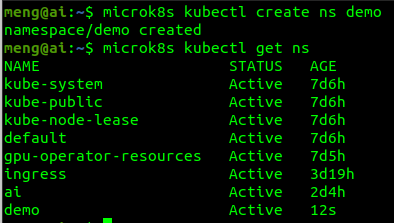
\includegraphics[width=\textwidth]{fig/ns-demo.png}

\item Label demo namespace \\
\textbf{kubectl label ns demo tier=test} \\
\newline
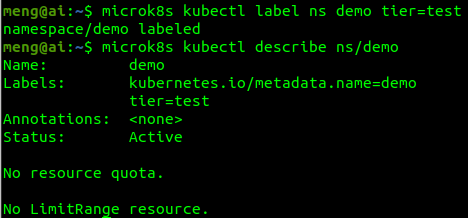
\includegraphics[width=\textwidth]{fig/demo-tier.png}

\item Create nginx-alpine deployment \\
\textbf{kubectl create deploy nginx-alpine \texttt{-{}-}image=nginx:alpine \texttt{-{}-}replicas=3 \texttt{-{}-}namespace=demo} \\
\newline
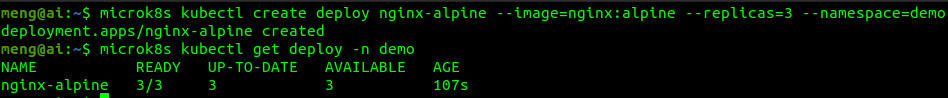
\includegraphics[width=\textwidth]{fig/nginx-deploy.png}

\item Label nginx-alpine deployment \\
\textbf{kubectl label deploy nginx-alpine app=nginx tag=alpine \texttt{-{}-}namespace=demo \texttt{-{}-}overwrite} \\
\newline
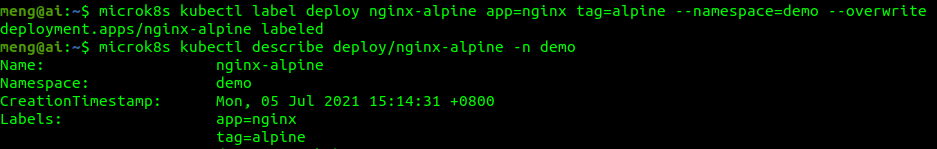
\includegraphics[width=\textwidth]{fig/nginx-app-tag.png}

\item Expose nginx-alpine deployment \\
\textbf{kubectl expose deploy/ngin-alpine \texttt{-{}-}port=8111 \texttt{-{}-}namespace=demo} \\
\newline
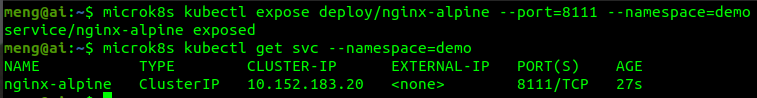
\includegraphics[width=\textwidth]{fig/nginx-svc.png}

\item Create config map \\
\textbf{kubectl create configmap nginx-version \texttt{-{}-}from-literal=version=alpine \texttt{-{}-}namespace=demo} \\
\newline
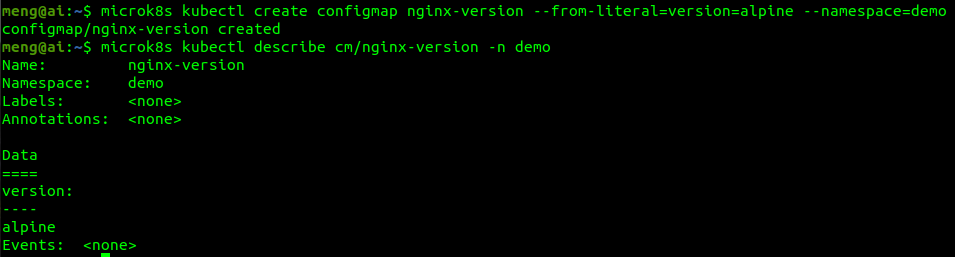
\includegraphics[width=\textwidth]{fig/nginx-config.png}

\end{enumerate}

\end{document}